\section*{Dati e risultati}

Nella prima parte dell'esperienza abbiamo calcolato il tempo caratteristico ($\tau$) del nostro circuito $R\,C$ per tre valori differenti sia di $R$, la resistenza del circuito che di $C$, la capacità del condensatore. Per essere sicuri dei valori di resistenza e di capacità utilizzati gli abbiamo misurati grazie al multimetro digitale. Nel resto della relazione saranno usati questi valori per elaborare i dati e non quelli nominali.

Noi sappiamo che per un circuito $R\,C$, nel quale tutti i componenti sono ohmici, la relazione che sussiste tra il tempo caratteristico ($\tau$), la resistenza ($R$) e il condenzatore ($C$) è la seguente:

\begin{equation}
	\tau \,=\, R\,C
	\label{eq:tau}
\end{equation}
%
Per avere un riscontro con i dati ricavati sfruttando la relazione (\ref{eq:tau}) abbiamo utilizzato l'oscilloscopio, correttamente tarato, per ottenere il valore del tempo caratteristico del circuito, leggendo il valore del tempo ad una determinata tensione. Sapendo che in un circuito $R\,C$ la diffrenza di potenziale in funzione del tempo segue la legge:

\begin{equation}
	V\ped{t} \,=\, V\ped{0}\,(1\,-\,e^{-\frac{t}{\tau}})
	\label{eq:potenziale}
\end{equation}
%
se calcoliamo la differenza di potenziale al tempo $\tau$ otteniamo che la tensione al tempo caratteristico vale esattamente:

\begin{equation}
	V\ped{\tau} \,=\, 0.632\,V\ped{0} 
\end{equation}
%
dove in entrambe le equazioni $V\ped{0}$ indica la differenza di potenziale in uscita dal generatore di funzioni d'onda, $t$ è il tempo e $\tau$ è il tempo caratteristico del circuito.

Quindi nella seguente tabella sono riportati i valori del tempo caratteristico ricavato teoricamente ($\tau\ped{teo}$) risolvendo l'equazione (\ref{eq:tau}), e quello ricavato dalla lettura dell'oscillosopio ($\tau\ped{exp}$).

\begin{table}[H]
  \centering
  \begin{tabular}{l | c c c}
      \multicolumn{4}{c}{\textbf{Tempo caratteristico $(\tau)$}} \\
      \toprule
      Resistenza $[\si{\ohm}]$ & Capacità $[\si{\farad}]$ & $\tau\ped{exp} [\si{\second}]$ & $\tau\ped{teo} [\si{\second}]$ \\
      \midrule
      $(499\,\pm\,1)$k   &  $(5.00\,\pm\,0.01)\times10^{-9}$ 	& $ (2.40\,\pm\,0.01)\cdot10^{-3}$ 		& $(2.4\,\pm\,0.1)\cdot10^{-3}$ \\
      $(19.9\,\pm\,0.1)$k  &  $(0.99\,\pm\,0.01)\cdot10^{-6}$ 		& $ (2.08\,\pm\,0.01)\times10^{-3}$ 	& $(1.9\,\pm\,0.1)\cdot10^{-3}$ \\
      $(997\,\pm\,1)$    &  $(99.3\,\pm\,0.1)\cdot10^{-9}$ 		& $ (1.04\,\pm\,0.01)\times10^{-3}$ 	& $(0.9\,\pm\,0.1)\times10^{-3}$ \\
      \bottomrule
  \end{tabular}
  \caption{In questa tabella sono riportati i valori del tempo caratteristico sia teorico $\tau\ped{teo}$ che sperimentale $\tau\ped{exp}$ in base ai vari valori di resistenze e capacità presenti nel nostro circuito. ([$\times$]: Ho vinto!!! [$\cdot$]: gneeeee!)}
  \label{tab:tris}
\end{table}

Infine abbiamo calcolato il valore della capacità, a priori incognita, di un condensatore. Questo è stato fatto risolvendo la semplice equazione:

\begin{equation}
	C \,=\, \frac{\tau}{R}
	\label{eq:cap}
\end{equation}
%
dove i valori di $R$ e $\tau$ sono noti in quanto la resistenza è stata impostata a piacere e il tempo caratteristico acquisito sperimentalmente grazie all'oscilloscopio.

\begin{SCfigure}[1][h]
    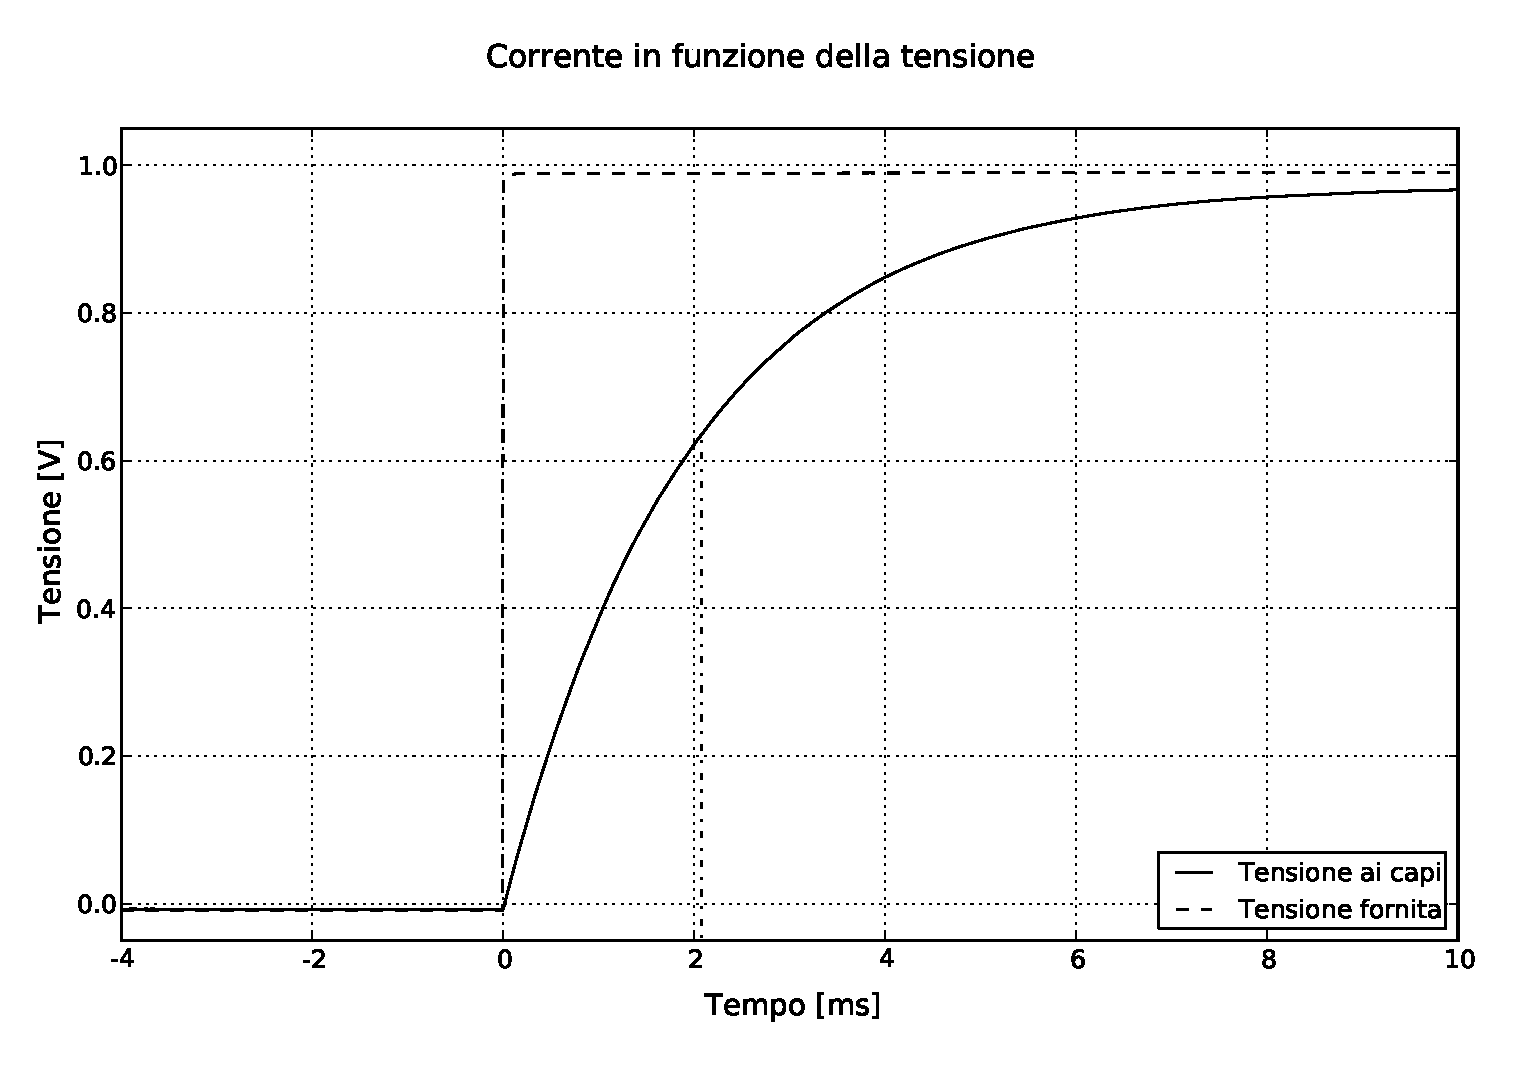
\includegraphics[width=140mm]{fig.pdf}
    \caption{La linea tratteggiata mostra l'andamento della tensione erogata dal generatore d'onde, mentre la linea continua
      rappresenta la tensione ai capi di uno dei condensatori in esame. È stata disegnata una linea punteggiata verticale che mostra il
      valore del tempo tipico del circuito RC.}
\end{SCfigure}
